\documentclass[a4paper,12pt]{article}
\usepackage[utf8]{inputenc}
\usepackage[T1]{fontenc}
\usepackage[french]{babel}
\usepackage[right=2.5cm, left=2.5cm]{geometry}
\usepackage[ddmmyyyy]{datetime}
\usepackage[table]{xcolor}
\usepackage{lmodern,mathptmx,changepage,titlesec,hyperref,listings,lstautogobble,graphicx,array,longtable,multirow,lipsum,tikz,shorttoc,enumitem}
\usetikzlibrary{arrows,automata}
\usetikzlibrary{positioning}

\renewcommand{\rmdefault}{\sfdefault} %Utilisation de la police sans-serif ("Computer Modern Sans") pour la police roman
\renewcommand{\ttdefault}{pcr} 	%Utilisation d'une police "CourrierNew" pour la police monospaced (pour faire un listing manuel)
\linespread{1.15}				%Interligne

%Utilisation de liens colorés en bleu et soulignés
\hypersetup{colorlinks=true, urlcolor=blue, urlbordercolor=blue, linkcolor=black, linkbordercolor=white}
\makeatletter \Hy@AtBeginDocument{\def\@pdfborder{0 0 1} \def\@pdfborderstyle{/S/U/W 1}}\makeatother

\titlespacing*{\section} {0cm}{7ex plus 1ex minus .2ex}{1.5ex plus .2ex}
\titlespacing*{\subsection} {0cm}{4.5ex plus 1ex minus .2ex}{1.5ex plus .2ex}
\titleformat*{\section}{\huge\bfseries}
\titleformat*{\subsection}{\Large\bfseries}
\titleformat*{\subsubsection}{\normalsize\bfseries}

\definecolor{darkgreen}{rgb}{0,0.8,0}
\definecolor{mygray}{rgb}{0.93,0.93,0.93}
\definecolor{mymauve}{rgb}{0.58,0,0.82}
\lstset{	
	basicstyle=\small\ttfamily,
	backgroundcolor=\color{mygray},
	breaklines=true,
	breakatwhitespace=true,
	postbreak=\raisebox{0ex}[0ex][0ex]{\ensuremath{\color{red}\hookrightarrow\space}},
	tabsize=3,
	frame=none,
	rulecolor=\color{black},
	keywordstyle=\color{blue}\bfseries,
	stringstyle=\color{orange},
	showstringspaces=false,
	commentstyle=\footnotesize\color{darkgreen},
	keepspaces=true,
	extendedchars=true,
	numbers=left,
	numberstyle=\tiny\color{lightgray},
	stepnumber=1,
	escapeinside={(@}{@)},
	autogobble=true,
	literate=
		{á}{{\'a}}1 {é}{{\'e}}1 {í}{{}}1 {ó}{{\'o}}1 {ú}{{\'u}}1
		{Á}{{\'A}}1 {É}{{\'E}}1 {Í}{{\'I}}1 {Ó}{{\'O}}1 {Ú}{{\'U}}1
		{à}{{\`a}}1 {è}{{\`e}}1 {ì}{{\`i}}1 {ò}{{\`o}}1 {ù}{{\`u}}1
		{À}{{\`A}}1 {È}{{\'E}}1 {Ì}{{\`I}}1 {Ò}{{\`O}}1 {Ù}{{\`U}}1
		{ä}{{\"a}}1 {ë}{{\"e}}1 {ï}{{\"i}}1 {ö}{{\"o}}1 {ü}{{\"u}}1
		{Ä}{{\"A}}1 {Ë}{{\"E}}1 {Ï}{{\"I}}1 {Ö}{{\"O}}1 {Ü}{{\"U}}1
		{â}{{\^a}}1 {ê}{{\^e}}1 {î}{{\^i}}1 {ô}{{\^o}}1 {û}{{\^u}}1
		{Â}{{\^A}}1 {Ê}{{\^E}}1 {Î}{{\^I}}1 {Ô}{{\^O}}1 {Û}{{\^U}}1
		{œ}{{\oe}}1 {Œ}{{\OE}}1 {æ}{{\ae}}1 {Æ}{{\AE}}1 {ß}{{\ss}}1
		{ç}{{\c c}}1 {Ç}{{\c C}}1 {ø}{{\o}}1 {å}{{\r a}}1 {Å}{{\r A}}1
		{€}{{e}}1 {£}{{\pounds}}1 {«}{{\guillemotleft}}1
		{»}{{\guillemotright}}1 {ñ}{{\~n}}1 {Ñ}{{\~N}}1 {¿}{{?`}}1
}

%Redéfinition de la taille de \Huge pour le titre du document
\makeatletter\renewcommand\Huge{\@setfontsize\Huge{37pt}{40}}\makeatother
\date{\today}

\title{\vspace{\fill}\textbf{\Huge Manuel utilisateur}}

\begin{document}
\pagenumbering{gobble}\clearpage
\maketitle\vspace{9em}
\begin{center}
\includegraphics[scale=3]{dcbrain.png}\end{center}
\begin{center}
\includegraphics[scale=0.7]{../Cahier/logo.png}\end{center}
\newpage
\tableofcontents
\newpage\clearpage\pagenumbering{arabic}

\section{Introduction}
	Cette application web est un outil de visualisation et d'analyse descriptive de données provenant de fichiers CSV structurés. Elle s'utilise via un navigateur web.
	
	L'utilisation des différentes fonctionnalités de l'application ainsi que le format des fichiers compatibles pour les traitements sont précisées dans ce document.
	
\section{Guide Pratique}
	\subsection{Étape 1 : sélection d'un fichier}
		La première étape est par réalisée par une fenêtre principale qui permet de charger un fichier CSV pour exécuter la visualisation et ensuite l'analyse descriptives de ses données. 
		
		Deux manières sont possibles pour le chargement du fichier.\\
		La première consistant à glisser le fichier dans la zone de drop comme le montre l'illustration suivante :
		
	\begin{center}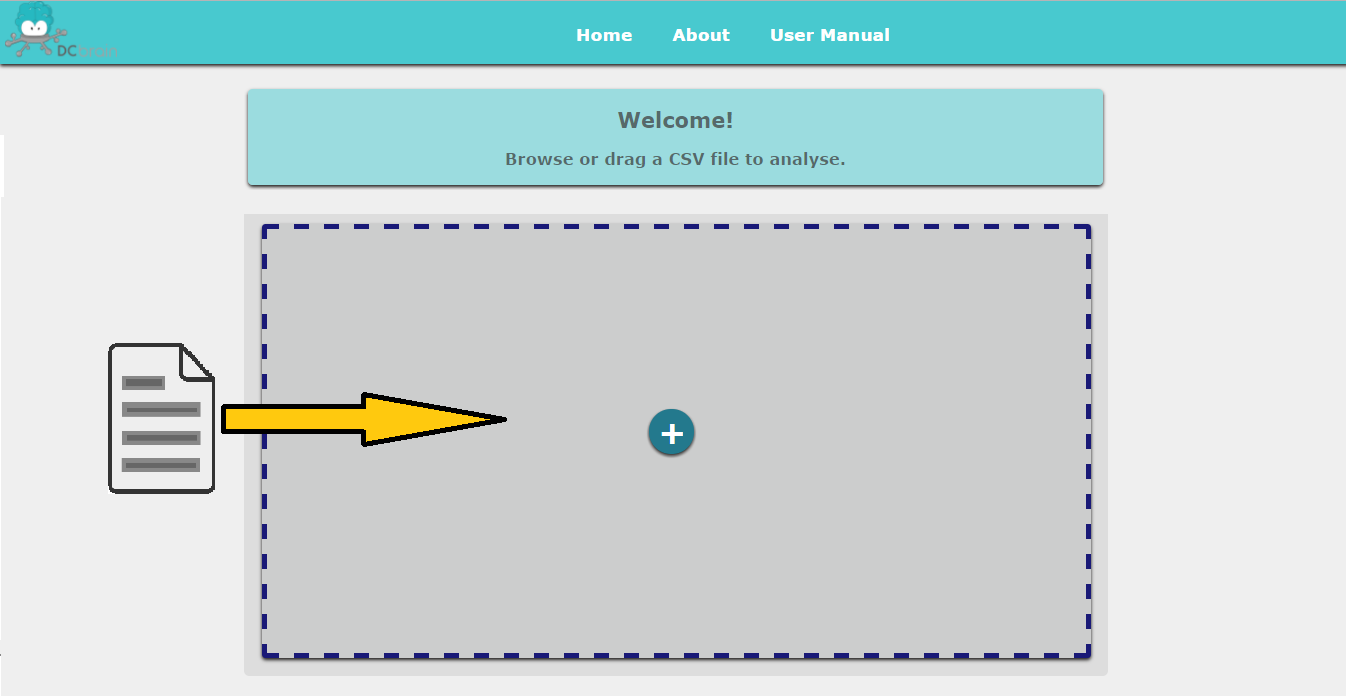
\includegraphics[scale=0.45]{fenetreDragDrop.png}\end{center}
		  
		 La seconde correspond à la méthode classique de parcours de l'arborescence de fichiers pour récupérer le fichier CSV, en cliquant sur l'icône \textbf{+} comme le montre l'illustration suivante :
		 
	\begin{center}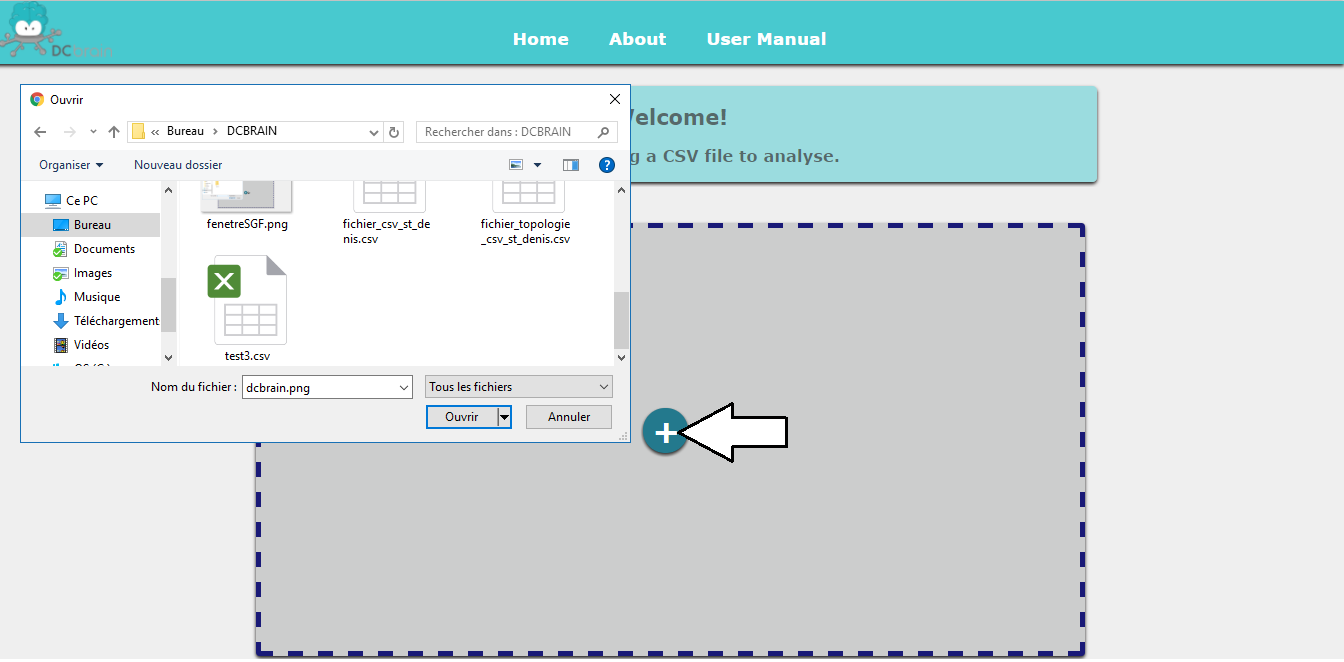
\includegraphics[scale=0.45]{fenetreSGF.png}\end{center}
	
		Le fichier sélectionné doit respecter certains critères pour pouvoir continuer vers la prochaine étape avec succès :
		\begin{itemize}
			\item Nom ne contenant pas d'espaces
			\item Extension \lstinline!.csv!
			\item Contenu lisible (non formaté)
			\item Contenu assez structuré : bien que l'application s'efforce de gérer des fichiers assez quelconques, il vaut mieux que leurs contenus soient assez structurés, c'est à dire, décrit par des colonnes aux types prédéfinies, et dans l'ordre suivant :
			\begin{itemize}
				\item timestamp : mois jour année, \lstinline!heure:minute:seconde!
				\item parent : index du nœud parent
				\item enfant : index du nœud enfant
				\item mesure (unité) : valeur
			\end{itemize}
		\end{itemize}
		Exemple :
		\begin{center}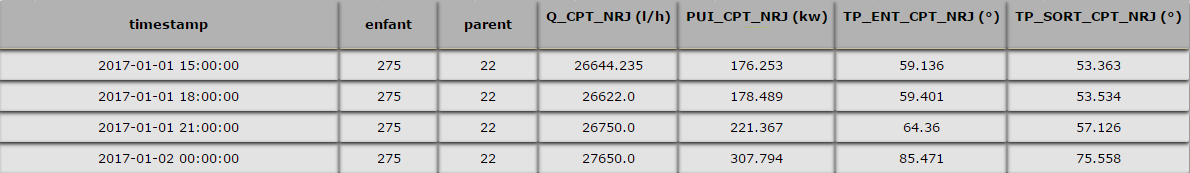
\includegraphics[scale=0.52]{exampleCSV.png}\end{center}
		
		Après avoir choisi un fichier, l'application va se rediriger vers une deuxième fenêtre si aucune erreur n'est détectée. Sinon, un message d'erreur s'affiche sur la fenêtre comme ci-dessous.
		
				
		\begin{center}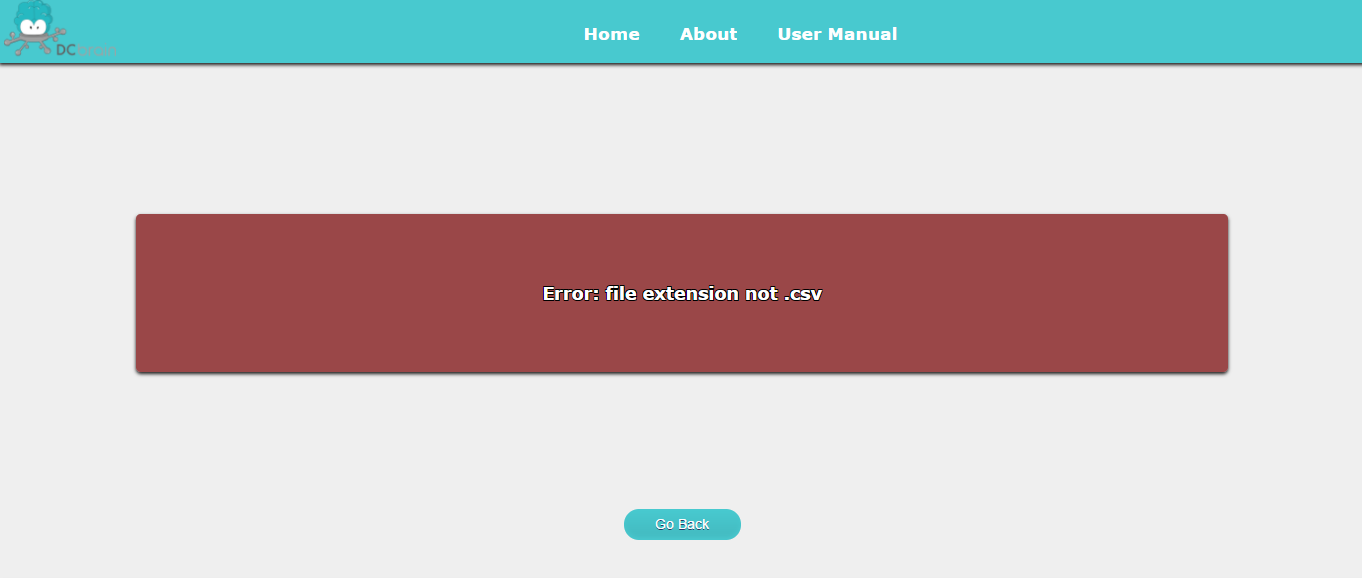
\includegraphics[scale=0.45]{fenetreErreur.png}\end{center}
			
	\subsection{Étape 2 : affichage, filtrage et choix des données}
		Cette étape permet à visualiser le contenu du fichier \lstinline!.csv! chargé précédemment. Si le format de ce fichier est bien respecté, on doit obtenir un résultat comme celui-ci :
		\begin{center}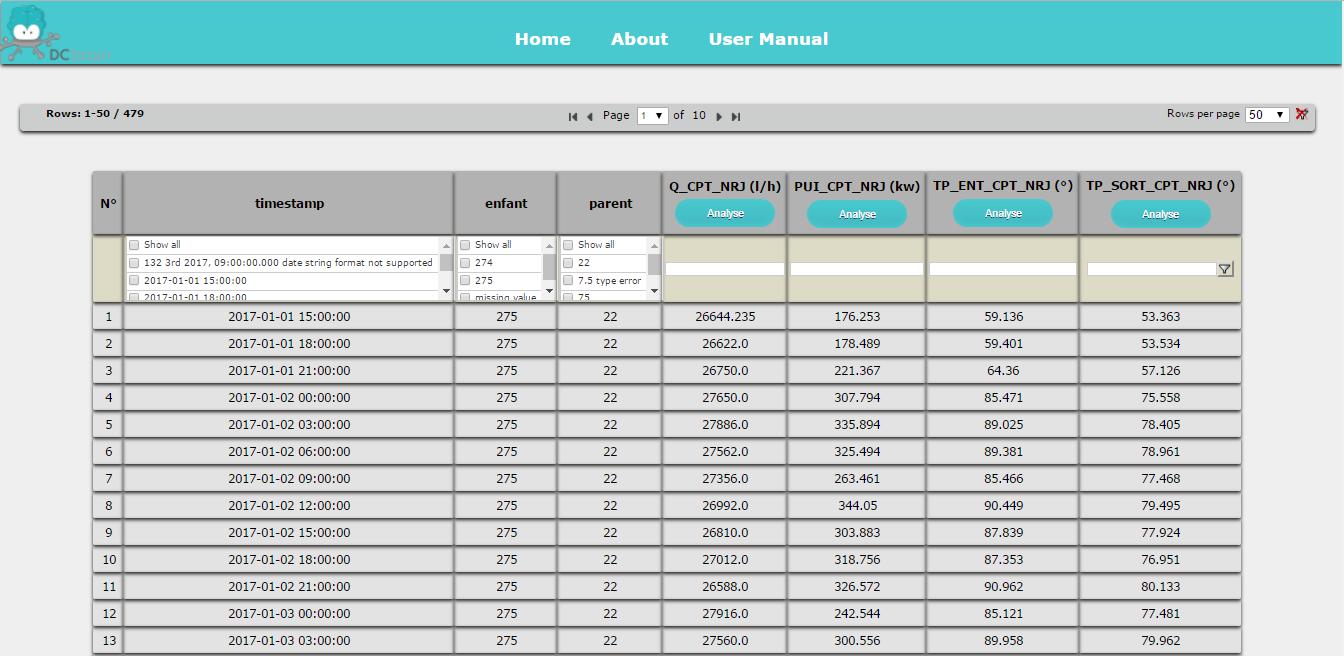
\includegraphics[scale=0.45]{fenetre2.png}\end{center}
		
		Une case contenant une donnée erronée ou manquante est surlignée en rouge pour l'indiquer à l'utilisateur. Une information sur l'erreur sera affichée lors du survol de cette case :
		
		\begin{center}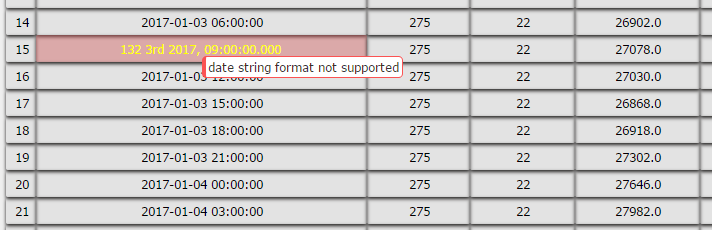
\includegraphics[scale=0.45]{fenetre2Erreur.png}\end{center}
		
		Les zones représentées ci-dessous contiennent les filtres applicables sur les données de chaque colonne (sélection d'un filtre ou recherche textuelle). Après le choix d'un filtre, l'affichage sera automatiquement mis à jour :
		
		\begin{center}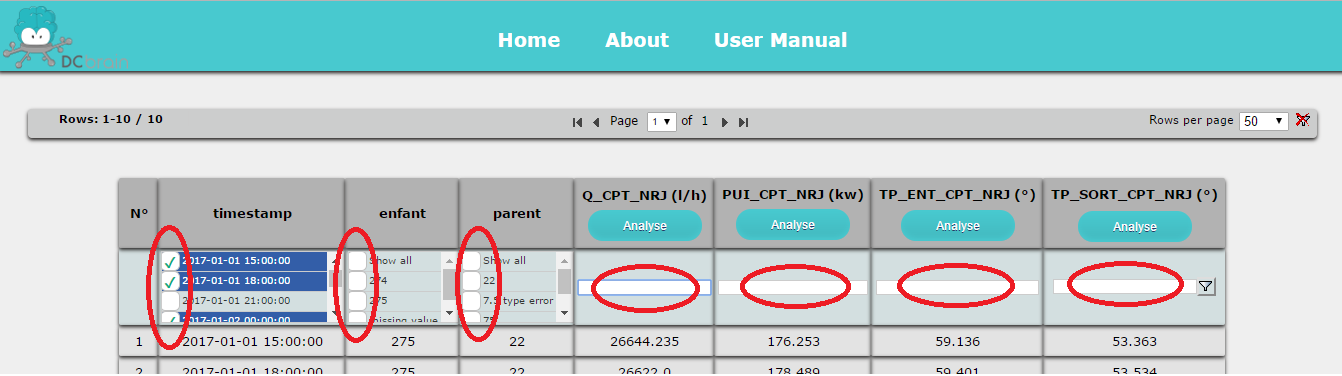
\includegraphics[scale=0.45]{fenetre2Filtre.png}\end{center}
		
		Dans la zone de recherche textuelle, des \textbf{filtres par plages de valeurs} sont possible, par l'utilisation des opérateurs suivants :
		
		\begin{center}\vspace{-1em}\footnotesize\begin{longtable}{|>{\centering}m{2cm}|>{\centering}m{9cm}|>{\centering\arraybackslash}m{3cm}|}			
			
			\hline \multicolumn{1}{|c|}{\textbf{Opérateur}} & \multicolumn{1}{c|}{\textbf{Description}} & \multicolumn{1}{c|}{\textbf{Exemple}}\\
			
			\hline	< & Valeurs inférieures à celle indiquée & < 1000\\
			\hline	<= & Valeurs inférieures ou égales à celle indiquée & <= 1000\\
			\hline	> & Valeurs supérieures à celle indiquée & > 1000\\
			\hline	>= & Valeurs supérieures ou égales à celle indiquée & >= 1000\\
			\hline	>= & Valeurs supérieures ou égales à celle indiquée & >= 1000\\
			\hline	! & Valeurs différentes de celle indiquée & !1000\\
			\hline	\&\& & ET logique & > 1000 \&\& < 2000\\
			\hline	|| & OU logique & < 1000 || > 2000\\
			\hline
			
		\end{longtable}\vspace{-1em}\end{center}
		
		Il est aussi possible de \textbf{renommer les colonnes} en cliquant sur leur nom.\\
		~\\
		Un bouton pour l'exécution de l'analyse descriptives de données sur colonne est disponible en dessous du nom de celui-ci :
		
		\begin{center}\includegraphics[scale=0.45]{fenetre2Analyse.png}\end{center}
		
		
	\subsection{Étape 3 : résultats de l'analyse}
		
		\begin{center}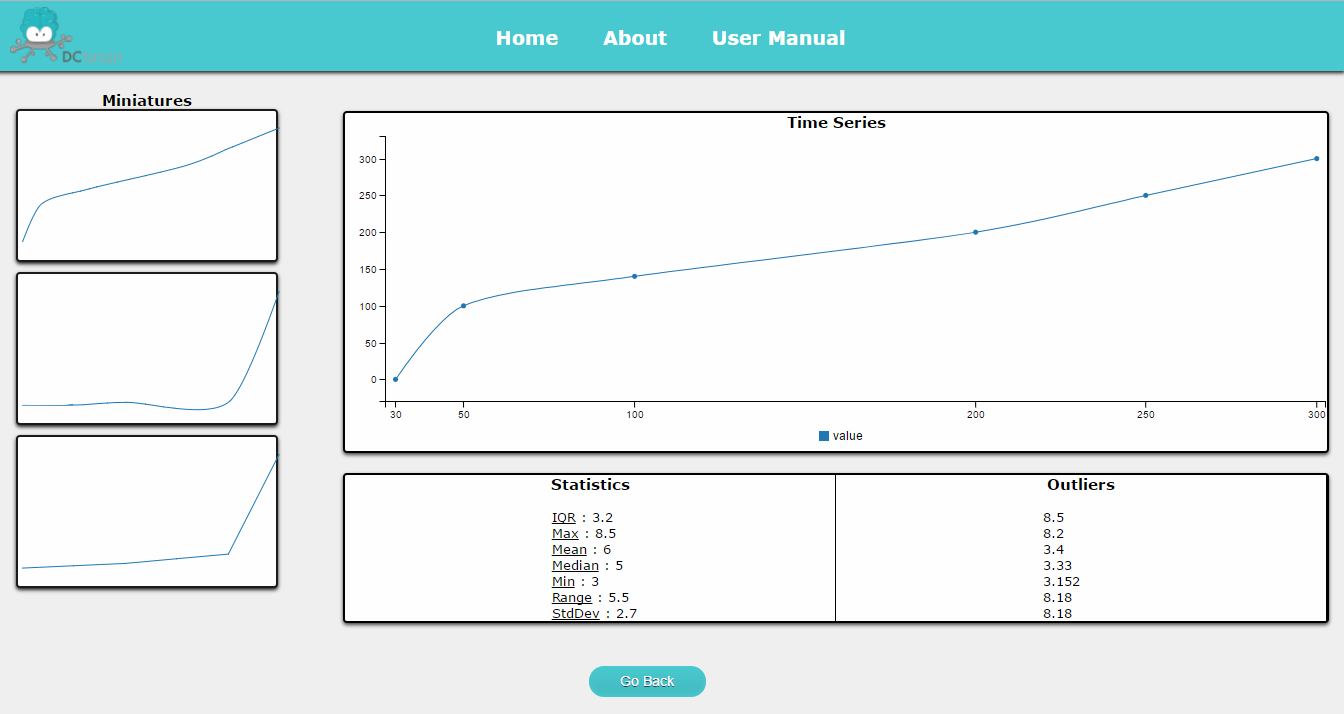
\includegraphics[scale=0.45]{fenetre3.png}\end{center}
			
		La fenêtre ci-dessus représente la dernière étape du traitement des données, l'étape de consultation des résultats d'analyse descriptive. Ces résultats sont constitués de deux catégories d'éléments :
		\begin{itemize}
			\item Des valeurs statistiques à consulter directement.
			\item Des représentations graphiques : il suffit de cliquer sur une miniature pour accéder à une vue précise et interactive du graphe sélectionné :
			\begin{center}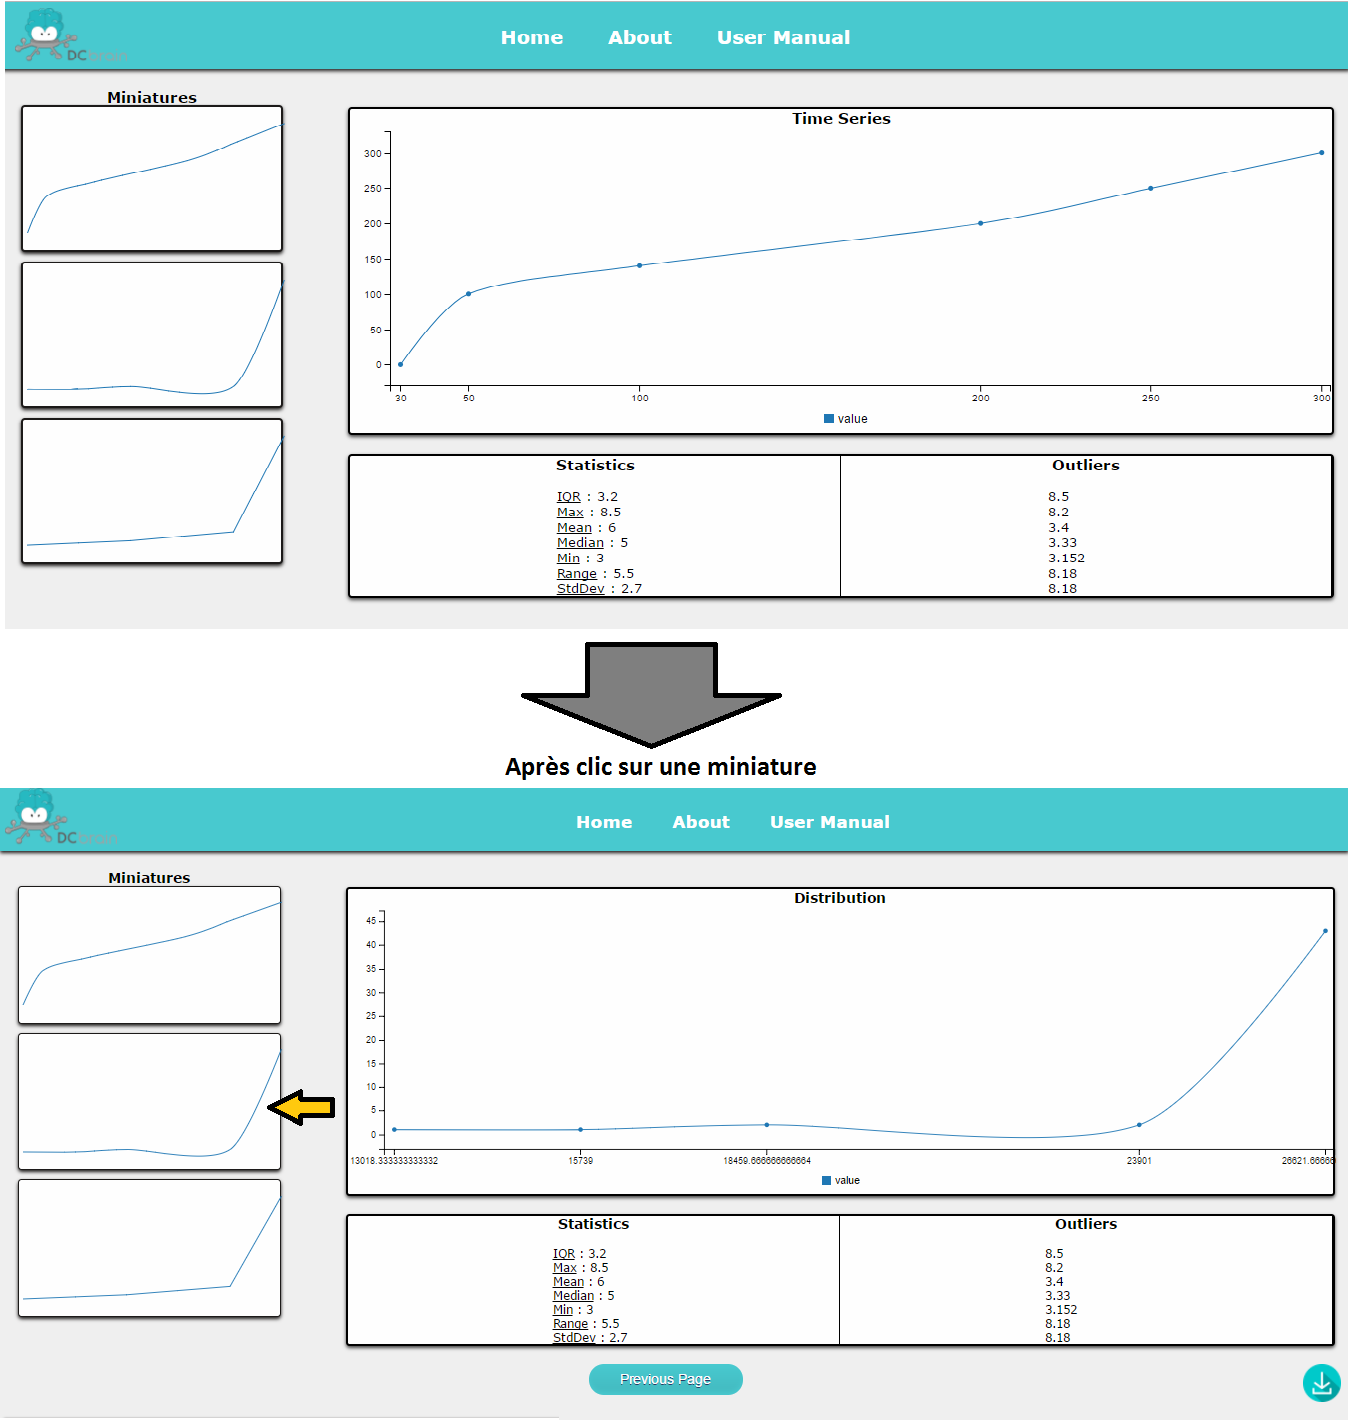
\includegraphics[scale=0.40]{fenetre3-2.png}\end{center}\vspace{4em}	
		\end{itemize}
		
		Pour le cas des séries temporelles, un graphe est disponible par arc différent. Afin de consulter la série temporelle voulue, il faut cliquer sur le bouton radio correspondant :
		\begin{center}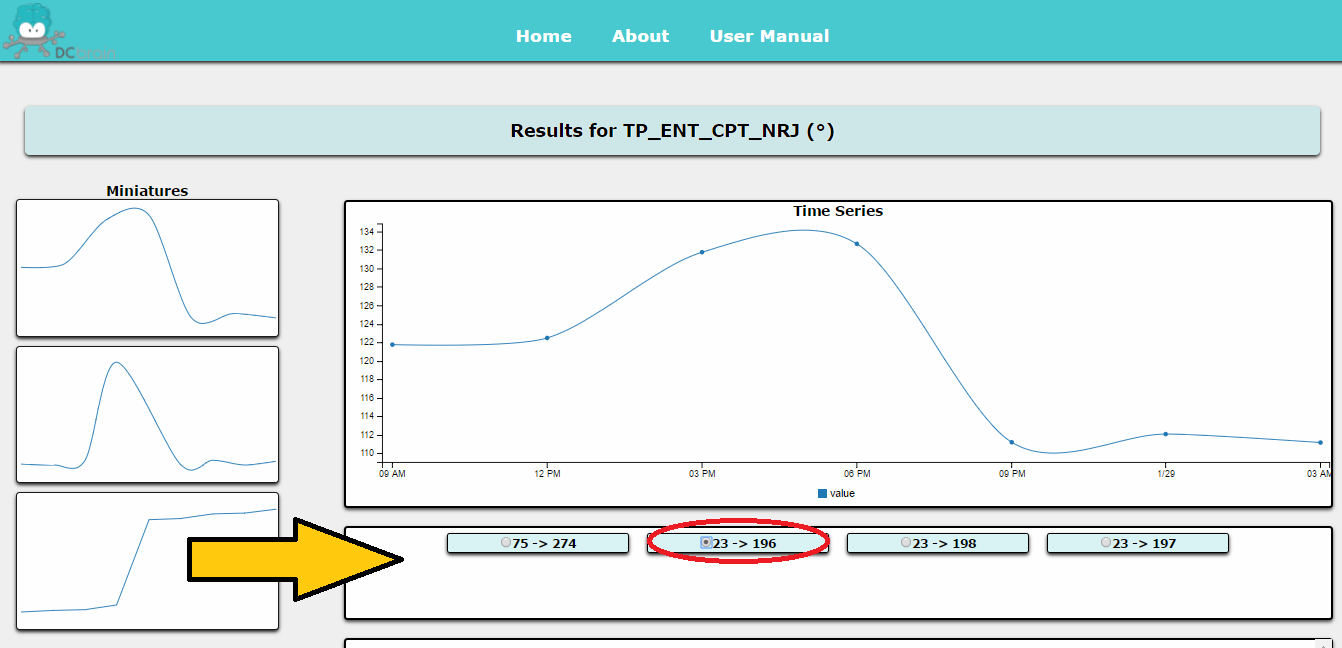
\includegraphics[scale=0.40]{fenetre3Arcs.png}\end{center}\vspace{4em}
		
		Une fonctionnalité de retour est disponible pour revenir à l'étape 2 et effectuer une autre analyse sans relancer l'application depuis le départ :
		\begin{center}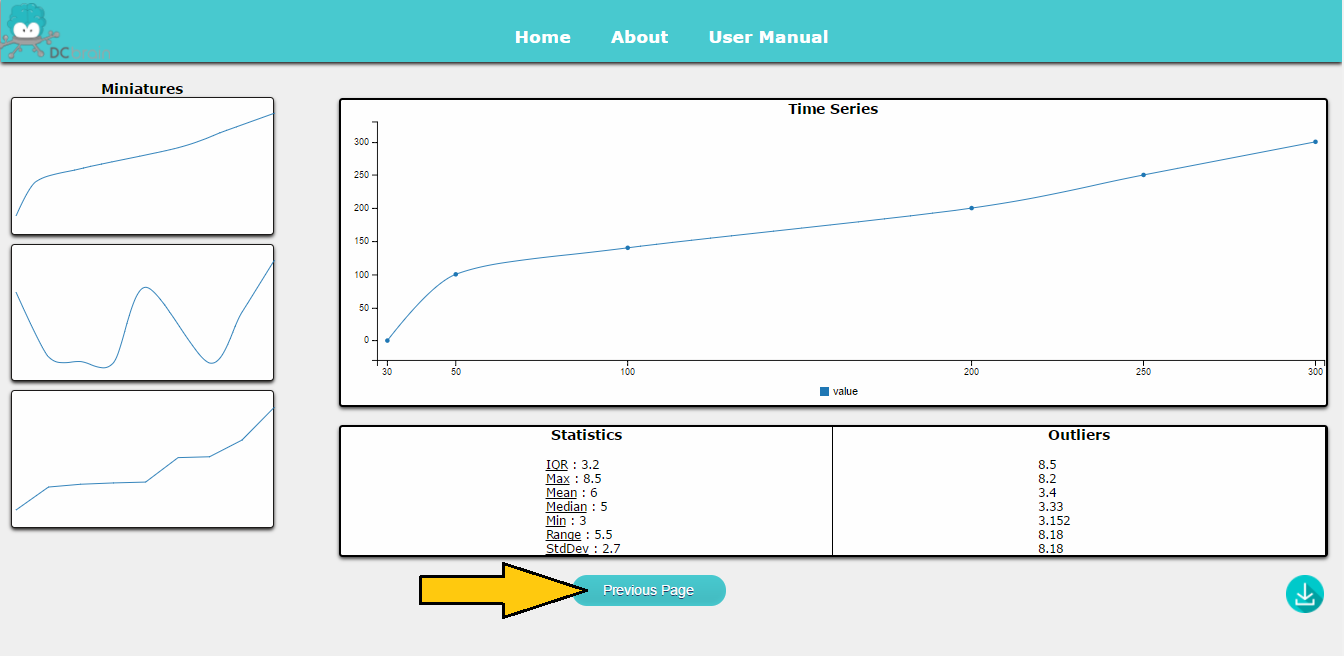
\includegraphics[scale=0.50]{fenetre3prec.png}\end{center}\vspace{4em}
			
		Enfin, il est possible d'exporter les résultats de l'analyse dans un fichier CSV grâce à une fonctionnalité de téléchargement :
		\begin{center}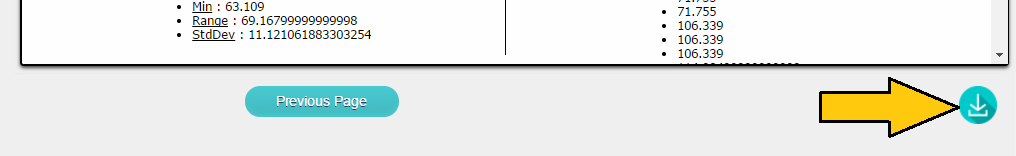
\includegraphics[scale=0.50]{fenetre3Download.png}\end{center}

\end{document}
